\documentclass[output=paper]{langsci/langscibook} 
\author{Manuel Widmer \affiliation{University of Zurich}} 

\markuptitle{Same same but different: on the relationship between egophoricity and evidentiality}{Same same but different: on the relationship between egophoricity and evidentiality}
\shorttitlerunninghead{Same same but different: egophoricity and evidentiality}

% \title{\texorpdfstring{Word formation and word history:\\ The case of
%  \textsc{capitalist} and \textsc{capitalism}}{Word formation and word
% history:  CAPITALIST and
% CAPITALISM}}

% \renewcommand{\lsCollectionPaperFooterTitle}{Word formation and word
% history: The case of  \noexpand\textsc{capitalist} and
% \noexpand\textsc{capitalism}}
 

\abstract{Egophoricity (a.k.a. “conjunct/disjunct”) is a grammatical phenomenon whose grammatical status has been discussed controversially in recent years. While some scholars have analyzed egophoricity as a subcategory of the well-established grammatical category \textit{evidentiality}, others have treated egophoricity as an independent grammatical category. This study aims at assessing the relationship between egophoricity and evidentiality from a functional-typological perspective. The chapter first discusses the varying structural complexity of egophoric systems against the backdrop of typological models that treat egophoricity as an evidential subcategory (e.g. \citealt{Plungian2010}; \citealt{SanRoqueLoughnane2012}). It is argued that such models fare well with complex egophoric systems of the Lhasa Tibetan type (see \citealt{TournadreDorje2003}) but fall short of accommodating binary egophoric systems of the Kathmandu Newar type (see \citealt{Hargreaves2005}). In a second step, the chapter takes a closer look at systems of the Lhasa Tibetan type, arguing that there are Lhasa Tibetan-type systems in which egophoric and allophoric markers display a considerable degree of independence, both from a functional and a structural point of view. These observations provide substantial evidence for the claim that egophoricity constitutes a functional domain distinct from evidentiality.}

\begin{document}
\maketitle

\section{Introduction}\label{s:mw1}

Egophoricity (a.k.a. conjunct/disjunct) is a cross-linguistically rare phenomenon that has so far only been documented for a comparatively small number of languages spoken in the Himalayas, the Caucasus, South America and Papua New Guinea (cf. \citealt{Creissels2008}). The grammatical status of egophoricity is a controversial issue that has been discussed in recent years. While some scholars have analyzed egophoricity as a subcategory of the well-established grammatical category \textit{evidentiality}, which serves the primary function of marking one’s source of information (\citealt{Aikhenvald2004}), others have maintained that egophoricity has a different functional motivation and should be considered as a grammatical category in its own right. This paper contrasts these two approaches, arguing that egophoricity and evidentiality are best conceived of as two independent grammatical categories but still interact with each other in various ways because they share a conceptually related functional motivation.

The chapter is structured as follows: §\ref{ex:mw2} discusses some terminological issues and gives a brief overview of different descriptive approaches towards egophoric systems. §\ref{ex:mw3} focuses on the distinction between egophoric systems consisting of two markers and egophoric systems comprising three or more markers. It is argued that binary systems cannot easily be reconciled with existing typologies of evidentiality, which suggests that egophoricity may in fact constitute a grammatical category distinct from evidentiality. §\ref{ex:mw4} further develops this argument by demonstrating that there are languages in which egophoricity and evidentiality manifest themselves as structurally independent subsystems. §\ref{ex:mw5} summarizes the results of this study and highlights some directions for further research.

\section{Preliminaries}\label{s:mw2}
\subsection{Terminology}\label{s:mw2-1}

What is referred to as \emph{egophoricity} in this chapter has been described under different names in the past. Initially, the phenomenon was known under the name “conjunct/disjunct”, a term that was introduced by \cite{HaleWatters1973} and subsequently popularized by \cite{Hale1980} and \cite{DeLancey1990}. Since the 1990s, various scholars have proposed a range of additional terms, either to refer to the phenomenon itself, its subcategories, or both. Table \ref{tab:mw1} below gives an overview of some terminological proposals (see \citealt{SanRoque2018} for a detailed overview).

\begin{table}
\begin{tabularx}{\textwidth}{llL{6cm}}
\hline
\textbf{Author}	&	\textbf{Cover term} 	&	\textbf{Subcategories}\\
\hline
\cite{Tournadre1991}	&	–	&	“egophoric”\newline vs.\newline “heterophoric”\newline	\\
\cite{Sun1993}	&	“person”	&	“self-person”\newline vs.\newline “other-person”\newline	\\
\cite{Haller2000}	&	“volitionality”	&	“volitional”\newline vs.\newline “non-volitional”\newline	\\
\cite{Huber2005} 	&	–	&	“old knowledge”\newline vs.\newline “new knowledge”\newline	\\
\cite{Creissels2008}	&	“assertor’s involvement marking”	&	“assertor’s involvement”	\\
\hline
\end{tabularx}
\caption{Selected terminological approaches to egophoricity}
\label{tab:mw1}
\end{table}	



The designation \emph{egophoricity}, which is derived from \citeauthor{Tournadre1991}’s (\citeyear{Tournadre1991}) \emph{egophoric}, has gained ever more acceptance in the course of the past decade and is now the most widely used term. The term “heterophoric”, which was introduced as an antonym of the term \emph{egophoric} by \cite{Tournadre1991}, never gained much currency in the literature. This is most probably due to the fact that \citeauthor{Tournadre1991} himself abandoned the term “heterophoric” early on when he gave up his dichotomous analysis of the Lhasa Tibetan egophoric system (cf. \citealt[301, fn. 48]{Tournadre2008}). However, various scholars have subsequently reintroduced antonyms to describe the antonymic value of \emph{egophoric} in binary egophoric systems. These antonyms are “non-egophoric” (\citealt{SanRoque2018}), “alterphoric” (\citealt{Post2013}), and “allophoric” (\citealt{Widmer2017a}). In what follows, the terms \emph{egophoric} and \emph{allophoric} are used to refer to the two subcategories of egophoricity.\footnote{Note that the terms \emph{egophoricity}, \emph{egophoric}, and \emph{allophoric} were already used by \cite{Dahl2000}, albeit in a different sense. \citeauthor{Dahl2000} does not use the term \emph{egophoricity} to refer to an epistemic grammatical phenomenon but to distinguish between two types of reference: \emph{egophoric reference} and \emph{allophoric reference}. The first includes reference to speech-act participants, generic reference, and logophoric reference, whereas the latter comprises all other types of reference.}

It is generally assumed that egophoric systems revolve around an epistemic role that comprises the different speech act roles to which the relevant markers may relate in different pragmatic contexts (see below for discussion). This epistemic role has been given a range of different names such as “locutor” (\citealt{Curnow1997}), “epistemic source” (\citealt{Hargreaves1991}, \citealt{Hargreaves2005}), “informant” (\citealt{BickelNichols2007}), or “assertor” (\citealt{Creissels2008}). The present chapter follows \cite{Creissels2008} in using the term \emph{assertor}.

\subsection{Approaches to egophoricity}\label{s:mw2-2}

In the course of the past decades, scholars have proposed different analyses of egophoricity. In early studies (e.g. \citealt{HaleWatters1973}; \citealt{Hale1980}), egophoricity was analyzed as a peculiar type of person agreement, an approach that has occasionally been invoked by recent typological work (e.g. \citealt{Aikhenvald2004}; \citealt{BickelNichols2007}). Person-based analyses have in common that they focus on the characteristic distribution of egophoric / allophoric markers in declarative and interrogative contexts (see Table \ref{tab:mw2} below), which they contrast with the distribution of person endings in ordinary person indexation systems.

\begin{table}
\begin{tabularx}{.80\textwidth}{XXX}
\hline
	&	\textbf{\textsc{declarative}}	& \textbf{\textsc{interrogative}}	\\
\hline
\textbf{\textsc{speaker}}	&	\textsc{ego}	&	\textsc{allo}	\\
\textbf{\textsc{addressee}}	&	\textsc{allo}	&	\textsc{ego}	\\
\textbf{\textsc{other}}	&	\textsc{allo}	&	\textsc{allo}	\\
\hline
\end{tabularx}
\caption{The prototypical distribution of egophoric / allophoric markers across clause types}
\label{tab:mw2}
\end{table}	

Whether or not it is feasible to treat egophoricity as a manifestation of the grammatical category \emph{person} essentially hinges on how one defines the concept \emph{person}. A traditional notion of person that is solely based on the roles \emph{speaker}, \emph{addressee}, and \emph{other} is not particularly useful for describing the distribution of egophoric and allophoric markers. However, within the framework of a broader definition that conceives of \emph{person} as “the grammaticalization of conceptual distinctions between participants involved in speech activities” (\citealt[220]{BickelNichols2007}), it is possible to establish a link between person agreement and egophoricity. Under such an approach, egophoric systems can be analyzed as person agreement systems that make a binary distinction between the assertor, viz. the speech act participant against whose knowledge a proposition is profiled, and everybody else (see \citealt{Bickel2008}; \citealt[223]{BickelNichols2007}; \citealt{Creissels2008}). However, this comes at the cost of blurring the fundamental distinction between syntactic agreement (determined by syntactic roles of arguments) and pragmatic agreement (determined by the identity of speech act participants and the type of speech act).

Person-based approaches towards egophoricity offer valuable insights into the different ways in which the participants of speech acts may be conceptualized across languages. At the same time, scholars working in such frameworks have often interpreted the assertor-based conceptualization of speech acts as the core function of egophoric systems. In other words, they have taken agreement with the assertor as the primary function of egophoricity (see \citealt{BickelNichols2007}; \citealt{Creissels2008}). This generalization is problematic for two reasons. First, a person-based analysis may work well for languages that have highly syntacticized egophoric systems, but it runs into difficulties when dealing with languages that have egophoric systems that are based on pragmatic rather than syntactic principles (cf. \citealt{SanRoque2018}). Second, there is some evidence that egophoric markers may not be invariably tied to the role of the assertor. One piece of evidence for this claim comes from the Chibchan languages Ika and Kogi. For both languages, \citeauthor{Bergqvist2012} (\citeyear{Bergqvist2012}, \citeyear{Bergqvist2016}) has described verbal affixes that are functionally reminiscent of egophoric / allophoric markers but appear to be sensitive to the speech act roles \emph{speaker} and \emph{addressee} rather than the epistemic role \emph{assertor}. Another piece of evidence comes from the Tibeto-Burman language Bunan. Bunan possesses the volitive suffixes -\textit{te} (\textsc{sg}) / -\textit{the} (\textsc{pl}), which indicate one’s intention to perform an action (\citealt[555--556]{Widmer2017a}). These suffixes are clearly modal in nature and accordingly have a different functional motivation than egophoric markers (see below for a discussion of that aspect). However, they still revolve around the epistemic role of the assertor (\citealt[453--459]{Widmer2017a}). These facts suggest that the epistemic role of the assertor is not a part of the functional definition of egophoricity but rather represents a distinct grammatical phenomenon that can occur independently of egophoric systems.

In sum, person-based analyses of egophoric systems are rarely propagated in the literature nowadays, most probably due to the analytical challenges outlined above. In contemporary studies, egophoricity is commonly analyzed as an epistemic phenomenon, that is to say, a grammatical means to relate the knowledge that is conveyed in a given speech act to speech act participants. These epistemic approaches can be broadly classified into two types: (i) those that conceive of egophoricity as a subcategory of evidentiality in the sense of \cite{Aikhenvald2004}, i.e. as having “source of information” as their primary meaning, and (ii) those that treat egophoricity as an epistemic category with a different functional motivation.

Approaches that treat egophoricity as a subcategory of evidentiality in a more or less explicit manner are encountered both in cross-linguistic and language-specific studies. Typological studies that have to be mentioned in this context are \cite{Plungian2010} and \cite{SanRoqueLoughnane2012}. \citeauthor{Plungian2010} (\citeyear[34]{Plungian2010}) postulates an evidential subcategory “participatory evidence”, which indicates that a speaker knows about an event because she / he was directly involved in it.\footnote{Note that \cite{Plungian2010} adopts the term \emph{participatory} evidence from \cite{Oswalt1986}.} Although this definition is reminiscent of the functional properties of egophoric markers, \citeauthor{Plungian2010} does not identify participatory evidence with egophoricity (which he refers to as “conjunct/disjunct”). Rather, he states that egophoric systems are “not so much related to the grammatical expression of evidentiality but to the expression of person (i.e. that of the speaker)” (43), thus suggesting that evidentiality and egophoricity are distinct categories. At the same time, he notes that the Trans-New Guinea language Oksapmin possesses participatory evidentials (34).
%page numbers?
Indeed, \cite{Loughnane2009} describes a “participatory-factual” or “personal-factual” evidential category for this language. However, \cite[253]{Loughnane2009} also explicitly compares this evidential subcategory to egophoric marking, stating that “[t]he conjunct [i.e. egophoric] term in conjunct/disjunct systems [i.e. egophoric systems] appears, at least in some languages, to be a personal evidential.” Accordingly, there is a link between \citeauthor{Plungian2010}’s (\citeyear{Plungian2010}) notion “participatory evidence” on the one hand and egophoric marking on the other, even though Plungian does not make this explicit.

In their survey of evidential systems in languages of the New Guinea Highlands, \cite{SanRoqueLoughnane2012} follow \cite{Plungian2010} in postulating an evidential subcategory “participatory evidence”, which is used to mark events that the speaker performed herself / himself or which are generally known to her / him. Unlike \cite{Plungian2010}, \citeauthor{SanRoqueLoughnane2012} explicitly link this category to egophoricity (which they call “conjunct/disjunct”), stating that the languages of the New Guinea Highlands “highlight the relevance of participatory and visual-sensory evidentials to conjunct/disjunct systems, and suggest that in certain cases “conjunct” and “disjunct” terms can be analyzed as participatory and visual(-sensory) evidentials, respectively” (\citeyear[158]{SanRoqueLoughnane2012}).

Another typologically oriented study that has to be mentioned in this context is a recent article by \cite{TournadreLaPolla2014}. Like \cite{Plungian2010} and \cite{SanRoqueLoughnane2012}, the two authors treat egophoricity as an evidential subcategory which they refer to as “egophoric” or “personal”. However, unlike the above cited authors, \cite{TournadreLaPolla2014} additionally extend \citeauthor{Aikhenvald2004}’s (\citeyear{Aikhenvald2004}) original definition of evidentiality from simply marking one’s “source of information” to marking both one’s “source and access to information”.

Some recent language-specific studies that analyze egophoricity as an evidential subcategory are \cite{Loughnane2009}, whose work has already been mentioned above, as well as \cite{Norcliffe2018} and \cite{Floyd2018}, who describe egophoric markers as a part of complex evidential systems of the Barbacoan languages Namtrik / Guambiano and Cha’palaa, respectively.

Approaches that treat egophoricity as an epistemic category with a functional motivation different from “source of knowledge” have so far predominantly applied in the description of individual languages, in particular languages spoken in the Greater Himalayan region. The following table gives an overview of these approaches.\footnote{It is important to note that these descriptive models differ strongly from each other in terms of terminology and the grammatical status that is assigned to egophoricity. Accordingly, it would be misleading to think of these different models as a unified approach. However, it is still justified to group them together since they all define egophoricity in a way that is not compatible with \citeauthor{Aikhenvald2004}’s (\citeyear{Aikhenvald2004}) definition of evidentiality.}

\begin{table}
\begin{tabularx}{\textwidth}{L{3.7cm}L{6.3cm}}
\hline
Language & Functional motivation\\
\hline 
Kathmandu Newar (\citealt[188]{Hargreaves1991}, \citeyear[31]{Hargreaves2005})\newline Bunan (\citealt[459]{Widmer2017a})	&	\mbox{privileged access to mental states / knowledge}\newline \mbox{vs.}\newline \mbox{non-privileged access to mental states / knowledge}	\\
Dzongkha (\citealt[112]{vanDriem1992})	&	\mbox{assimilated / personal knowledge}\newline \mbox{vs.}\newline \mbox{acquired / objective knowledge}	\\
Shigatse Tibetan (\citealt[88]{Haller2000})\newline Themchen Tibetan (\citealt[136]{Haller2004})\newline Kaike (\citealt[304]{Watters2006})	&	\mbox{volitional acting}\newline \mbox{vs.}\newline \mbox{non-volitional acting}	\\
Mangghuer (\citealt[194]{Slater2003})	&	\mbox{high degree of speaker involvement}\newline \mbox{vs.}\newline \mbox{low degree of speaker involvement}	\\
Kyirong Tibetan (\citealt[98]{Huber2005})	&	\mbox{old knowledge}\newline \mbox{vs.}\newline \mbox{new knowledge}	\\
Galo (\citealt[123]{Post2013})	&	\mbox{internal knowledge}\newline \mbox{vs.}\newline \mbox{external knowledge}	\\
Tsafiki (\citealt{Dickinson2016})	&	\mbox{knowledge inside one’s territory of information}\newline \mbox{vs.}\newline \mbox{knowledge outside one’s territory of information}	\\
\hline
\end{tabularx}
\caption{Non-evidential epistemic approaches towards egophoricity}
\label{tab:mw3}
\end{table}	

As the table illustrates, most of the above cited approaches characterize the functional motivation of egophoricity in terms of a binary contrast between two different types of knowledge, viz. privileged / personal / old / internal knowledge vs. non-privileged / objective / new / external knowledge. While individual approaches focus on different functional aspects of this dichotomy, it is clear that they essentially all describe the same phenomenon, viz. an epistemic grammatical category that is conceptually related yet functionally distinct from evidentiality (in the sense of \citealt{Aikhenvald2004}) and distinguishes between two types of perspectives on knowledge: an epistemically privileged and epistemically non-privileged perspective.
 
\section{Different manifestations of egophoricity}\label{s:mw3} 

In the languages of the world, we encounter two different structural manifestations of egophoric systems. First, there are binary egophoric systems, which instantiate a dichotomic contrast between an egophoric and an allophoric marker. Such a system can for example be found in Kathmandu Newar (Tibeto-Burman, Nepal). The endings of the Kathmandu Newar egophoric system are illustrated in Table \ref{tab:mw4} below.

\begin{table}
\begin{tabularx}{.70\textwidth}{XXX}
\hline
& \textbf{\textsc{ego}} & \textbf{\textsc{allo}}\\
\hline
\textbf{\textsc{npst}} & -\textit{e} & -\textit{i}\\
\textbf{\textsc{pst}} & -\textit{ā} & -\textit{a}\\
\hline
\end{tabularx}
\caption{The Kathmandu Newar system (\citealt{Hargreaves2005})}
\label{tab:mw4}
\end{table}

Second, there are egophoric systems in which egophoric markers directly contrast with two or more evidential markers. Such a system has for example been described for Lhasa Tibetan, whose imperfective and perfective endings are illustrated in Table \ref{tab:mw5} below.\footnote{The egophoric markers -\textit{pa yin} and -\textit{byung} are tied to different participant roles. The first expresses an epistemically privileged perspective in combination with agents, while the latter expresses an epistemic privileged perspective in combination with undergoers (\citealt{WidmerZuniga2017}). The relevance of participant roles for egophoricity is not discussed in the detail in the present chapter but only briefly touched upon in § \ref{s:mw6}.}

\begin{table}
\begin{tabularx}{.90\textwidth}{XXXX}
\hline
	&	\textbf{\textsc{ego}}	&	\textbf{\textsc{direct}}	&	\textbf{\textsc{indirect}}	\\
\hline
\textbf{\textsc{ipfv}}	&	-\textit{gyi yod}	&	-\textit{gyis}	&	-\textit{gyi} \textit{yod}-\textit{pa red}	\\
\textbf{\textsc{pfv}}	&	-\textit{pa yin} / -\textit{byung}	&	-\textit{song}	&	-\textit{pa red}	\\
\hline
\end{tabularx}
\caption{The Lhasa Tibetan system (\citealt{DeLancey1990})}
\label{tab:mw5}
\end{table}
%\footnote{The egophoric markers -pa yin and -byung are tied to different participant roles. The first expresses an epistemically privileged perspective in combination with agents, while the latter expresses an epistemic privileged perspective in combination with undergoers (Widmer \& Zúñiga 2017). The relevance of participant roles for egophoricity is not discussed in the detail in the present chapter but only briefly touched upon in § 6.}

It is this variability in the structural organisation of egophoric systems that has given rise to controversies about the grammatical status of egophoricity and its relationship to evidentiality (cf. \citealt[295–296]{Widmer2017b}). The interpretation of egophoric markers as evidentials is sensible and practical from the perspective of ternary systems of the Lhasa Tibetan type, in which an egophoric marker like the imperfective ending -\textit{gyi yod} directly contrasts with the direct evidential ending -\textit{gyis} and the indirect evidential ending -\textit{gyi yod}-\textit{pa} red. However, such an evidential analysis is more difficult to uphold for a binary system of the Kathmandu Newar type, where one only encounters a binary contrast between the egophoric markers -\textit{e} (\textsc{npst}) / -\textit{ā} (\textsc{pst}) and the allophoric markers -\textit{i} (\textsc{npst}) / -\textit{a} (\textsc{pst}). Consider the following sentences from Kathmandu Newar below.

\begin{exe}
	\ex Kathmandu Newar, Tibeto-Burman\label{ex:mw1}
	\begin{xlist}
		\ex \label{ex:mw1a}
		\gll ji	wan-\textbf{ā}.\\
		1\textsc{sg} go-\textsc{pst}.\textbf{\textsc{ego}}\\
		\trans ‘I went.’ (\citealt[12]{Hargreaves2005})
		\ex \label{ex:mw1b}
		\gll ji	mhiga then-\textbf{a}.\\
		1\textsc{sg} yesterday arrive-\textsc{pst}.\textbf{\textsc{allo}}\\
		\trans ‘I arrived yesterday.’ (\citealt[13]{Hargreaves2005})
		\ex \label{ex:mw1c}
		\gll cha	 wan-\textbf{a}.\\
		2\textsc{sg} go-\textsc{pst}.\textbf{\textsc{allo}}\\
		\trans ‘You went.’ (\citealt[12]{Hargreaves2005})
		\ex \label{ex:mw1d}
		\gll wa	wan-\textbf{a}.\\
		3\textsc{sg} go-\textsc{pst}.\textbf{\textsc{allo}}\\
		\trans ‘S/he went.’ (\citealt[12]{Hargreaves2005})
	\end{xlist}
\end{exe}

As the examples illustrate, the egophoric ending -\textit{ā} is used whenever the assertor describes an event that she / he intentionally and consciously performed herself / himself, while the allophoric form -\textit{a} is used whenever the assertor describes an event that she did not instigate intentionally and / or consciously or that was performed by some other person. \citeauthor{Hargreaves1991} (\citeyear{Hargreaves1991}, \citeyear{Hargreaves2005}) has argued that egophoric and allophoric endings in Kathmandu Newar essentially encode an opposition of “privileged access” vs. “non-privileged access” to the mental state that is associated with intentional actions. Egophoric markers indicate that the assertor willfully instigated the event in question, while allophoric markers indicate that this is not the case.

Hargreaves’ analysis can be contrasted with the evidential approaches mentioned in § \ref{s:mw2-2}, which analyze egophoricity as an evidential subcategory usually referred to as “participatory evidence” (\citealt{Plungian2010}; \citealt{SanRoqueLoughnane2012}). If one were to apply such a descriptive approach to the Kathmandu Newar system, egophoric markers would have to be analyzed as evidential markers that mark a proposition as being based on knowledge that was acquired through personal participation in the relevant event.

As far as egophoric markers are concerned, such a model can be implemented without difficulties, as it provides an adequate functional characterization of egophoric marking. However, matters become more complex once we turn to allophoric markers. If we consider the Kathmandu Newar egophoric system presented in Table \ref{tab:mw4} as an evidential system and analyze the endings -\textit{e} ‘\textsc{npst.ego}’ and -\textit{ā} ‘\textsc{pst.ego}’ as expressing “participatory evidence”, we also have to come up with an adequate functional characterization of the contrasting endings -\textit{i} ‘\textsc{npst.allo}’ and -\textit{a} ‘\textsc{pst.allo}’. Egophoric and allophoric endings stand in a salient functional opposition and constitute a functionally self-contained system within the verbal domain. If the egophoric endings are analyzed as evidential markers, it appears conclusive that the corresponding allophoric endings should also be assigned an evidential function. However, such an analysis poses difficulties, as it is hard to assign clear evidential semantics to these markers. It is misleading to characterize allophoric endings as direct evidentials, as they can be used in contexts in which the assertor did not directly witness an event. At the same time, it is problematic to describe allophoric endings as indirect evidentials, since they can occur in contexts in which the assertor directly observed an event.

Current typological models of evidentiality are not helpful in resolving this issue. Consider the following table, which gives an overview of the typological models proposed by \cite{Aikhenvald2004}, \cite{Plungian2010}, \cite{SanRoqueLoughnane2012}, and \cite{Hengeveld2015}.

\begin{table}
\begin{tabularx}{.90\textwidth}{XXXX}
\hline
\textbf{\cite{Aikhenvald2004}}	&	\textbf{\cite{Plungian2010}}	&	\textbf{\cite{SanRoqueLoughnane2012}}	&	\textbf{\cite{Hengeveld2015}}	\\
\hline
–	&	Participatory	&	Participatory	&	–	\\
Visual	&	Visual	&	Visual	&	Event perception	\\
Sensory	&	Non-visual	&	Non-visual	&	Event perception	\\
Inference	&	Inferential	&	Results	&	Deduction	\\
Assumption	&	Presumptive	&	Reasoning	&	Inference	\\
Hearsay	&	Reported	&	Reported	&	Reportativity	\\
Quotative	&	Reported	&	Reported	&	Reportativity	\\
\hline
\end{tabularx}
\caption{Selected typological models of evidentiality}
\label{tab:mw6}
\end{table}

None of the models listed above postulates an evidential subcategory that accurately characterizes the function of allophoric forms in Kathmandu Newar or other languages with binary egophoric systems. Most notably, \cite{Plungian2010} and \cite{SanRoqueLoughnane2012}, which postulate participatory evidence as an evidential subcategory and apply this notion to markers that have been described as egophoric elsewhere in the literature, do not postulate another evidential subcategory that would correspond to the allophoric forms in binary egophoric systems. To be sure, \cite[158]{SanRoqueLoughnane2012} argue that allophoric endings appear to be functionally equivalent to “visual(-sensory)” evidentials in certain languages. However, as noted above, the allophoric endings of Kathmandu Newar cannot be described as direct evidentials. One might maintain an evidential analysis by augmenting \cite{Plungian2010} and \citeauthor{SanRoqueLoughnane2012}’s (\citeyear{SanRoqueLoughnane2012}) models with an additional allophoric / “non-participatory” evidential subcategory. However, as discussed earlier, this subcategory would be difficult to define with respect to its evidential value. These considerations illustrate that it is difficult to maintain an evidential analysis of allophoric endings and, more generally, of a binary egophoricity contrast of the Kathmandu Newar type.

Proponents of an evidential approach towards egophoricity might argue that allophoric markers could be analyzed as “non-evidential” forms that do not express any epistemic semantics. Such an analysis, however, is at odds with the fact that allophoric markers serve an epistemic function in the sense that they express the assertor’s non-privileged epistemic perspective with regard to an event. One might further argue that the epistemic construal of allophoric forms only arises as a consequence of a generalized conversational implicature (see \citealt{Levinson2000}), that is to say, because they stand in direct contrast with egophoric forms. However, such a pragmatic explanation would presuppose that allophoric forms are semantically less marked than egophoric forms. This asymmetric relationship would be expected to consistently manifest itself in terms of both form (the allophoric category is morphologically less marked than egophoric category) and / or function (the egophoricity distinction is neutralized in favor of the allophoric form in certain contexts) across languages. However, there is no compelling cross-linguistic evidence for a privative semantic markedness relationship between the domains of egophoric and allophoric marking.

In sum, binary egophoric systems pose a challenge to evidential approaches. If one analyzes egophoric markers as expressing “participatory evidence”, one is confronted with the difficulty that allophoric markers, which constitute an integral part of binary egophoric systems, cannot be adequately described under such an analysis. This observation suggests that egophoricity may not be an evidential category in the sense of \cite{Aikhenvald2004} but rather represents a functionally independent epistemic “package” that can be combined with an evidential system, as the example of Lhasa Tibetan demonstrates. If this assumption were correct, however, we would expect this functional independence to correlate with a certain degree of structural independence in ternary systems of the Lhasa Tibetan type. This hypothesis is further explored in §\ref{s:mw4} below.

\section{Structural evidence for an independent status of egophoricity}\label{s:mw4}
\subsection{Egophoricity as an independent functional domain}\label{s:mw4-1}

There are languages with ternary egophoric systems of the Lhasa Tibetan type in which egophoricity and evidentiality manifest themselves as independent functional domains. Such a system is for example attested in Bunan, a Tibeto-Burman language of North India. The language possesses a simple egophoric system in the present tense, in which there is a binary contrast between an egophoric and an allophoric form, and a more complex ternary system in the past tense, in which the egophoric form is part of paradigm that also comprises evidential markers. Table \ref{tab:mw7} and the example sentences in (\ref{ex:mw2}) illustrate the present tense endings.

\begin{table}
\begin{tabularx}{.60\textwidth}{L{.8cm}L{.8cm}XX}
\hline
&	&	\textbf{\textsc{ego}}	&	\textbf{\textsc{allo}}	\\
\hline
\multirow{2}{*}{\textbf{\textsc{prs}}} & \textbf{\textsc{sg}}	&	-\textit{ek}	&	-\textit{are}	\\
& \textbf{\textsc{pl}}	&	-\textit{$^h$ek}	&	-\textit{$^h$ak}	\\
\hline
\end{tabularx}
\caption{The present tense egophoric system of Bunan (\citealt{Widmer2017a})}
\label{tab:mw7}
\end{table}

\begin{exe}
	\ex Bunan, Tibeto-Burman\label{ex:mw2}
	\begin{xlist}
		\ex \label{ex:mw2a}
		\gll gi	dzamen noj dza-k-\textbf{ek}.\\
		1\textsc{sg} food much eat-\textsc{intr}-\textbf{\textsc{prs}.\textsc{ego}.\textsc{sg}}\\
		\trans ‘I am eating a lot.’ (Widmer fieldnotes)
		\ex \label{ex:mw2b}
		\gll han / tal dzamen noj dza-k-\textbf{are}.\\
		2[\textsc{sg}] / 3[\textsc{sg}]	food much eat-\textsc{intr}-\textbf{\textsc{prs}.\textsc{allo}.\textsc{sg}}\\
		\trans ‘You are eating a lot.’ / ‘She / he is eating a lot.’ (Widmer fieldnotes)
	\end{xlist}
\end{exe}

Table \ref{tab:mw8} and the example sentences in (\ref{ex:mw3}) illustrate the past tense endings.\footnote{The egophoric past tense marker has the allomorphs -\textit{et} \~ -\textit{men}, whereas the allophoric inferential past tense marker has the allomorphs -\textit{dʑi} (\textsc{sg}) / -\textit{tɕʰok} (\textsc{pl}) \~ -\textit{ta}. The allomorphs are lexically conditioned and depend on the transitivity class of the relevant predicate. Verbs belonging to the intransitive and middle class take the allomorphs -\textit{et} and -\textit{dʑi} (\textsc{sg}) / -\textit{tɕʰok} (\textsc{pl}), while verbs belonging to the transitive class take the allomorphs -\textit{men} and -\textit{ta}.}

\begin{table}
\begin{tabularx}{.9\textwidth}{L{.8cm}L{.8cm}X XXX}
\hline
	&		&	\textbf{\textsc{ego}}	&	\multicolumn{3}{c}{\textbf{\textsc{allo}}}					\\
	&		&		&	\textbf{\textsc{dir}}	&	\multicolumn{2}{c}{\textbf{\textsc{infer}}}		\\
\hline
\multirow{2}{*}{\textbf{\textsc{pst}}}	&	\textbf{\textsc{sg}}	&	\multirow{2}{*}{-\textit{et } \sim -\textit{men}}	&	-\textit{dza}	&	-\textit{dʑi}	&	\multirow{2}{*}{\sim -\textit{ta}}	\\
	&	\textbf{\textsc{pl}}	&		&	-\textit{ts$^h$a}	&	-\textit{tɕ$^h$ok}	&		\\
\hline
\end{tabularx}
\caption{The past tense egophoric system of Bunan (\citealt{Widmer2017a})}
\label{tab:mw8}
\end{table}

\begin{exe}
	\ex Bunan, Tibeto-Burman\label{ex:mw3}
	\begin{xlist}
		\ex 
		\gll gi dzamen noj dza-\textbf{et}.\\
		1\textsc{sg} food much eat-\textbf{\textsc{pst}.\textsc{ego}}\\
		\trans ‘I ate a lot.’ (Widmer fieldnotes)
		\ex 
		\gll han / tal dzamen noj dza-dza.\\
		2[\textsc{sg}] / 3[\textsc{sg}] food much eat-\textbf{\textsc{pst}.\textsc{allo}.\textsc{dir}.\textsc{sg}}\\
		\trans ‘You / she / he ate a lot.’ (The speaker witnessed the relevant event.) (Widmer fieldnotes)
		\ex 
		\gll han / tal dzamen noj dza-dʑi.\\
		2[\textsc{sg}] / 3[\textsc{sg}] food much eat-\textbf{\textsc{pst}.\textsc{allo}.\textsc{infer}.\textsc{sg}}\\
		\trans ‘You / she / he has eaten a lot.’ (The speaker infers that the relevant event must have taken place.) (Widmer fieldnotes)
	\end{xlist}
\end{exe}

As Table \ref{tab:mw9} illustrates, \cite{Widmer2017a} proposes a layered analysis of the past tense system, with an evidentiality distinction being nested inside an egophoricity distinction. This is not the only possible analysis of this past tense paradigm, however. Non-nested approaches towards structurally similar systems have been proposed in the literature as well (cf. \citealt{TournadreDorje2003}, \citeyear{Tournadre2008}; \citealt{SanRoqueLoughnane2012}; \emph{inter alia}). Under a non-layered approach, the egophoric form directly contrasts with a direct evidential and an inferential form. The non-layered analysis of the Bunan past tense system is illustrated in Table \ref{tab:mw9}.

\begin{table}
\begin{tabularx}{.9\textwidth}{L{.8cm}L{.8cm}X XXX}
\hline
	&		&	\textbf{\textsc{ego}}	&	\textbf{\textsc{dir}}	&	\multicolumn{2}{c}{\textbf{\textsc{infer}}}			\\
\hline
\multirow{2}{*}{\textbf{\textsc{prs}}}	&	\textbf{\textsc{sg}}	&	\multirow{2}{*}{-\textit{et} \sim -\textit{men}}	&	-\textit{dza}	&	-\textit{dʑi}	&	\multirow{2}{*}{\sim -\textit{ta}}	\\
	&	\textbf{\textsc{pl}}	&		&	-\textit{ts$^h$a}	&	-\textit{tɕ$^h$ok}	&		\\\hline
\end{tabularx}
\caption{A non-layered analysis of the Bunan past tense system}
\label{tab:mw9}
\end{table}

At first, a non-layered analysis of the Bunan system seems more parsimonious, as it allows one (i) to reduce the number of epistemic subcategories in the past tense from four to three and (ii) to reduce the number of epistemic categories from two to one. However, on closer examination it becomes clear that this analysis poses a number of difficulties in the case of Bunan.

If one adopts a non-layered approach and postulates \emph{egophoric} (\textsc{ego}), \emph{direct} (\textsc{dir}), and \emph{inferential} (\textsc{infer}) as directly contrasting values, it becomes impossible to relate the past tense system to the present tense system, which merely distinguishes the values \emph{egophoric} (\textsc{ego}) and \emph{allophoric} (\textsc{allo}). In particular, such an approach fails to explain how the value \textit{allophoric} relates to the values \textit{direct} and \textit{inferential}. Since a non-layered analysis presupposes that all of the aforementioned markers stand in a direct functional contrast, it entails that the values \textit{egophoric}, \textit{allophoric}, \textit{direct}, and \textit{inferential} all belong to the same functional domain. However, this analysis is at odds with the structural organization of the system, in which the values \textit{allophoric} and \textit{direct} / \textit{inferential} are in complementary distribution. In order to maintain a non-layered analysis, one would have to argue that the egophoric markers are “semantically hybrid” in the sense that they can both contrast with evidential markers, which specify one’s source of knowledge, as well as with allophoric markers, which express one’s epistemic outside perspective with regard to a certain event. However, this entails that egophoricity has to be defined as a “fuzzy” semantic concept, as its subcategory \textit{egophoric} can serve two different functions depending on the grammatical context in which it occurs. A non-layered approach towards egophoricity in Bunan thus raises a number of difficulties that can be avoided if one considers egophoricity and evidentiality as two distinct categories that are independent of each other but stand in a layered relationship.

It is important to note that the paradigm described in Table \ref{tab:mw8} is not the only paradigm in which egophoricity and evidentiality manifest themselves as two distinct functional domains. A structurally similar system is attested in the assumptive present tense, which occurs in propositions that are based on one’s overall knowledge of the world. In the assumptive present tense, the egophoricity distinction is nested inside of the evidential subcategory rather than the other way around. This is illustrated by the following table.

\begin{table}
\begin{tabularx}{.6\textwidth}{L{.8cm}L{.8cm}XX}
\hline
	&		&	\multicolumn{2}{c}{\textbf{\textsc{assum}}}			\\
	&		&	\textbf{\textsc{ego}}	&	\textbf{\textsc{allo}}	\\
\hline
\multirow{2}{*}{\textbf{\textsc{prs}}}	&	\textbf{\textsc{sg}}	&	\multirow{2}{*}{-\textit{men}}	&	-\textit{mendʑi}	\\
	&	\textbf{\textsc{pl}}	&		&	-\textit{mentɕ$^h$ok}	\\
\hline
\end{tabularx}
\caption{The assumptive present tense endings}
\label{tab:mw10}
\end{table}

The following sentences illustrate the use of the assumptive present tense.

\begin{exe}
	\ex Bunan, Tibeto-Burman\label{ex:mw4}
	\begin{xlist}
		\ex \label{ex:mw4a}
		\gll gun	eraŋ=maŋ mu noj ra-\textbf{men}.\\
		winter 1\textsc{pl}.\textsc{incl}=\textsc{all} snow much come-\textbf{\textsc{assum}.\textsc{ego}}\\
		\trans ‘In winter, there is a lot of snow in Lahaul.’ (\citealt[477]{Widmer2017a})
		\ex \label{ex:mw4b}
		\gll gun	eraŋ=maŋ mu noj ra-\textbf{mendʑi}.\\
		winter 1\textsc{pl}.\textsc{incl}=\textsc{all} snow much come-\textbf{\textsc{assum}.\textsc{allo}.\textsc{sg}}\\
		\trans ‘In winter, there is a lot of snow in Lahaul.’ (\citealt[477]{Widmer2017a})
	\end{xlist}
\end{exe}

The difference between the egophoric ending -\textit{men} and the allophoric ending -\textit{mendʑi} is so subtle that it is difficult to capture it in the English translation. The use of the egophoric ending indicates that the speaker makes this statement on the basis of knowledge that she / he considers to be personal and intimate. The use of the allophoric ending, in turn, indicates that the speaker makes this statement on the basis of knowledge that she / he considers to be equally accessible to other persons.

The assumptive present tense historically derives from a periphrastic construction consisting of the infinitive -\textit{men} and an inflected form of the equative copula \textit{jen}-. The originally periphrastic nature of the construction can still be seen in negated contexts. When the assumptive evidential present tense is negated, the equative copula occurs as a separate phonological word and expresses the negation.\footnote{In Bunan, verbal negation is commonly expressed by the prefix \textit{ma}-, which attaches to the verb root (\citealt[429--432]{Widmer2017a}). In the case of the equative copula \textit{jen}-, the negative prefix has phonologically fused with the copula, yielding the negative copula stem \textit{men}-.} Consider the following example.

\begin{exe}
	\ex Bunan, Tibeto-Burman\label{ex:mw5}\\
	\gll khjak ra-\textbf{men} \textbf{men} manɖi=astok ra-\textbf{men}.\\
	here	 come-\textbf{\textsc{inf}} \textbf{\textsc{neg}.\textsc{eq}.\textsc{ego}} Mandi=\textsc{term} come-\textbf{\textsc{assum}.\textsc{ego}}\\
	\trans ‘(These trees) do not grow here (in Kullu), they can be found up to Mandi.’ (\citealt[223]{Widmer2017a})
\end{exe}


Accordingly, one might argue that assumptive evidentiality in Bunan cannot be considered as an evidential subcategory in its own right, as the relevant construction is still partly periphrastic in negative contexts. However, in affirmative contexts the nonfinite verb form and the copula have phonologically fused to the extent that native speakers are no longer aware that the form originally consisted of two independent syntactic constituents. From a strictly synchronic point of view, it is thus legitimate to analyze the endings -\textit{men}, -\textit{mendʑi}, and -\textit{mentɕ$^h$ok} as nonsegmentable morphemes.

One might further argue that the notion of layeredness in itself is not a sufficient criterion to distinguish between the functional domains of egophoricity and evidentiality, as evidential subcategories can themselves display a layered structure. The Tibetan variety spoken in Spiti, North India, for example, displays a set of perfect markers that combine the semantics of direct perception evidentials with the semantics of inferential evidentials. Consider the following examples:

\begin{exe}
	\ex Spiti Tibetan, Tibeto-Burman\label{ex:mw6}
	\begin{xlist}
	\ex \label{ex:mw6a}
	\gll khō	 ārāk tʰūŋ-\textbf{wanuk}\\
	3\textsc{sg}	 liquor drink-\textsc{perf}.\textbf{\textsc{infer}.\textsc{vis}}\\
	\trans ‘He must have had liquor.’ (I can see it) (\citealt[46]{Hein2001})
	\ex \label{ex:mw6b}
	\gll khō pētɕā sīl-\textbf{anak}\\
	3\textsc{sg} book read-\textsc{perf}.\textbf{\textsc{infer}.\textsc{nonvis}}\\
	\trans ‘He must have read the book.’ (I can hear it) (\citealt[46]{Hein2001})
	\end{xlist}
\end{exe}


However, it appears that layered constructions like the one illustrated in (\ref{ex:mw6}), in which one grammatical form simultaneously expresses two different evidential subcategories, are rare and combinatorial possibilities of such constructions are highly restricted. These restrictions appear to be a consequence of the fact that two evidential subcategories have to relate to conceptually compatible information sources in order to complement each other. For example, it is difficult to imagine how a direct evidential contrast of visual vs. non-visual evidence could be nested inside of an assumptive evidential construction because the two subcategories presuppose conceptually distinct information sources, viz. one’s sensory perception and one’s overall knowledge of the world. One’s overall knowledge of the world cannot be accessed through any of one’s five senses. Accordingly, there is no cognitive basis for implementing a direct evidential contrast inside of an assumptive evidential construction.

Egophoricity, in turn, does not appear to be restricted in the same way and can be combined with evidential subcategories that presuppose different types of information sources. As has been demonstrated above, egophoricity oppositions can host evidential contrasts that presuppose the direct perception of an event (i.e. direct evidence) or the resultant state of an event (i.e. inferential evidence) and they can also be nested inside of evidential subcategories that presuppose world knowledge about an event. One could of course argue that egophoricity is combinable with so many different evidential subcategories because it presupposes an unspecific type of information source. However, given the fact that there is independent evidence that egophoricity constitutes an autonomous functional domain that is distinct from evidentiality, it is much more sensible to assume that egophoricity is so versatile because it does not indicate the source of one’s knowledge but rather specifies the quality of one’s knowledge in terms of a binary distinction between an epistemically privileged and an epistemically non-privileged perspective.

\subsection{Egophoricity as an independent morphological category}\label{s:mw4-2}

In the languages of the world, we also encounter epistemic systems in which egophoricity and evidentiality manifest themselves as morphologically independent subsystems. Such a system has been reported for the Barbacoan language Tsafiki, which displays two different sets of morphemes to encode egophoricity and evidentiality. As a consequence, the Tsafiki systems looks like a ternary system of the Lhasa Tibetan type from a functional perspective but differs from the latter in so far as egophoricity and evidentiality are realized as distinct morphological categories. This is illustrated in (\ref{ex:mw7a}) through (\ref{ex:mw7c}) below. In these examples, the markers -\textit{yo} ‘\textsc{ego}’ and -\textit{i} ‘\textsc{allo}’ occur in the morphological slot after the verb root, while the inferential evidential marker -\textit{nu} ‘\textsc{infer}’ occurs in the morphological slot following them.

\begin{exe}
	\ex Tsafiki, Barbacoan\label{ex:mw7}
	\begin{xlist}
	\ex \label{ex:mw7a}
	\gll la kuchi=ka tote-\textbf{yo}-e.\\
	1\textsc{masc} pig=\textsc{acc} kill-\textbf{\textsc{ego}}-\textsc{decl}\\
	\trans ‘I killed the pig.’ (\citealt[412]{Dickinson2000})
	\ex \label{ex:mw7b}
	\gll la kuchi=ka tote-\textbf{i}-e.\\
	1\textsc{masc} pig=\textsc{acc} kill-\textbf{\textsc{allo}}-\textsc{decl}\\
	\trans ‘I killed the pig (unintentionally).’ (\citealt[412]{Dickinson2000})
	\ex	\label{ex:mw7c}
	\gll la kuchi=ka tote-\textbf{i}-\textbf{nu}-e.\\
	1\textsc{masc} pig=\textsc{acc} kill-\textbf{\textsc{allo}}-\textbf{\textsc{infer}}-\textsc{decl}\\
	\trans ‘I must have killed the pig (unintentionally).’ (\citealt[412]{Dickinson2000})
	\end{xlist}
\end{exe}

In these examples, the egophoric marker -\textit{yo} ‘\textsc{ego}’ expresses that the assertor intentionally and consciously killed the pig, whereas the use of the allophoric marker -\textit{i} indicates that the assertor caused the animal’s death by accident. Within the domain of allophoric marking, there is an additional distinction between direct and inferential evidence. The presence of the inferential marker -\textit{nu} in (\ref{ex:mw7b}) suggests that the assertor did not directly witness the pig’s death but only infers what has happened upon finding the animal’s dead body, while the absence of the inferential marker in (\ref{ex:mw7c}) indicates that the assertor observed the animal’s death (cf. \citealt[412]{Dickinson2000}). The combination of the egophoric marker -\textit{yo} ‘\textsc{ego}’ and the inferential marker -\textit{nu} is not allowed (\citealt[410--413]{Dickinson2000}). This restriction does not come as a surprise, however. If a predicate takes an egophoric marker, this presupposes that the speaker directly witnessed the respective events. In other words, the privileged epistemic perspective that is implied by egophoric marking entails direct perception of the relevant facts.

One might argue that syntagmaticity is not a valid argument to distinguish the two categories because syntagmatic relationships may also hold between evidential markers (cf. \citealt{Aikhenvald2004}; \citealt{Hengeveld2015}) and egophoric markers (cf. \textit{Widmer2017a}; \citealt{Floyd2018}). However, the claim being made here is not that markers belonging to the same epistemic category should not be able to stand in a syntagmatic relationship with each other. Rather, the point is that one would expect to find systems in which egophoricity and evidentiality are encoded separately if the two categories were conceptually independent grammatical phenomena, and this is exactly what one encounters in Tsafiki.

\section{Discussion}\label{s:mw5}

The preceding sections have discussed the relationship between egophoricity and evidentiality from a structural perspective and argued that there is substantial evidence for the claim that egophoricity constitutes a grammatical category in its own right. The arguments that have been brought forward in favor of this position focus on different aspects of egophoric systems. §\ref{s:mw3} explores the functional motivation of egophoricity by contrasting \citeauthor{Hargreaves2005}’ (\citeyear{Hargreaves2005}) analysis of the Kathmandu Newar egophoric system with an alternative “evidential approach”. The section argues that such systems cannot be adequately described in terms of an evidential framework and makes a case for \citeauthor{Hargreaves2005}’ (\citeyear{Hargreaves2005}) analysis, under which egophoricity can be conceived of as a distinct epistemic category with a different functional motivation. §\ref{s:mw4-1} discusses the structural organization of complex epistemic systems that combine egophoric / allophoric and evidential markers. It is demonstrated that egophoricity and evidentiality constitute two functional layers in Bunan. These layers closely interact but are ultimately independent of each other. §\ref{s:mw4-2} adduces further evidence for that claim by discussing the case of Tsafiki, a language in which egophoricity and evidentiality stand in a syntagmatic relationship, constituting two independent morphological subsystems.

When considered in isolation, each of the three aspects discussed above may not provide sufficient evidence to warrant the analysis of egophoricity as a grammatical category different from evidentiality. However, when taken altogether, they make a compelling case for treating egophoricity as a grammatical category in its own right. After all, egophoricity meets the minimal requirements to be considered as an autonomous grammatical category. First, egophoricity manifests itself as a functionally and formally self-contained grammatical subsystem in languages with binary egophoric systems (e.g. Kathmandu Newar). Second, egophoricity may manifest itself as a self-contained grammatical subsystem in languages with complex epistemic systems. This may either be in the form of an autonomous functional domain (as in Bunan) or in the form of autonomous morphological system (as in Tsafiki).

One could make an even stronger case for treating egophoricity as an autonomous grammatical category if one were able to demonstrate that egophoricity and evidentiality categories combine into paradigms in which they constitute two orthogonal grammatical categories whose subcategories can be freely combined. Such a hypothetical paradigm is given in Table \ref{tab:mw11} below.

\begin{table}
\begin{tabularx}{.8\textwidth}{L{2cm}L{.8cm}XXX}
\hline
	&		&	\multicolumn{3}{c}{\textbf{Evidentiality}}					\\
	&		&	\textbf{\textsc{dir}}	&	\textbf{\textsc{infer}}	&	\textbf{\textsc{assum}}	\\
\hline
\multirow{2}{*}{\textbf{Egophoricity}}	&	\textbf{\textsc{ego}}	&	…	&	…	&	…	\\
	&	\textbf{\textsc{allo}}	&	…	&	…	&	…	\\
\hline
\end{tabularx}
\caption{A paradigm with egophoricity and evidentiality as orthogonal categories}
\label{tab:mw11}
\end{table}

However, evidence from natural languages suggests that egophoricity and evidentiality do not combine into paradigms in which they stand in an orthogonal relationship. Rather, it appears that egophoricity and evidentiality represent two distinct yet closely related functional domains that can combine into a number of different hierarchical relationships with each other. Evidence for this claim comes from the epistemic systems of Bunan and Tsafiki, which have been described in §\ref{s:mw4-1} and §\ref{s:mw4-2}. In both languages, we encounter an egophoric system in which the allophoric domain hosts an additional evidential contrast between \textit{direct} vs. \textit{inferential}. This is illustrated in Figure \ref{fig:mw1} below.

\begin{figure}
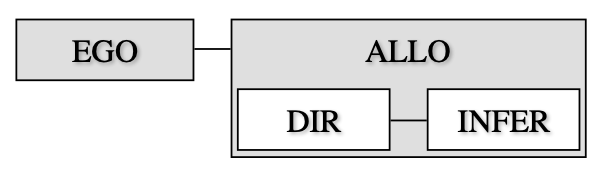
\includegraphics[width=.8\textwidth]{figures/widmer-1.png}
\caption{An egophoric system hosting an evidentiality distinction}
\label{fig:mw1}
\end{figure}

In Bunan, we additionally encounter an evidential subcategory hosting an egophoric system. This is illustrated in Figure \ref{fig:mw2} below.

\begin{figure}
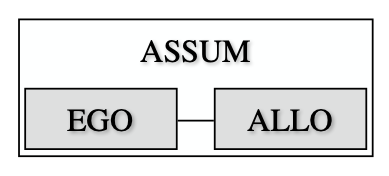
\includegraphics[width=.6\textwidth]{figures/widmer-2.png}
\caption{An evidential subcategory hosting an egophoric system}
\label{fig:mw2}
\end{figure}

The fact that egophoricity and evidentiality fail to combine into paradigms in which they represent orthogonal categories is a consequence of their closely related semantics. Both categories essentially serve the primary function of relating the knowledge that is conveyed in propositions to specific speech act participants. However, they diverge with regard to which aspect of this knowledge relation they profile. Egophoricity specifies the quality of one’s knowledge in terms of a dichotomic opposition that distinguishes between an epistemically privileged and an epistemically non-privileged perspective, while evidentiality specifies the source of one’s knowledge. 

The relationship between egophoricity and evidentiality is thus comparable to the relationship between the well-established grammatical categories tense and aspect (\citealt[299]{Widmer2017b}). In some of the world’s languages, temporal and aspectual distinctions are intertwined in such complex ways that it is difficult to tease them apart. At the same time, there is compelling cross-linguistic evidence that tense and aspect are two distinct grammatical phenomena, even though they may not be recognizable as such in all languages of the world. Accordingly, few scholars would argue that one should abandon the distinction between tense and aspect and, for example, treat aspect as a subcategory of tense or vice versa. In my view, the relationship between egophoricity and evidentiality should be conceptualized in the same manner. In some languages, egophoricity and evidentiality may be formally and functionally integrated in one single system to the extent that there is no reason to analyze them as separate phenomena. When describing such languages, it may be feasible and justified to describe egophoricity and evidentiality as exponents of one unified grammatical subsystem. However, when treating such languages from a cross-linguistic perspective, it is necessary to make a clear distinction between egophoricity and evidentiality, as there is compelling cross-linguistic evidence that they constitute two distinct grammatical phenomena. That is not to say that egophoricity and evidentiality should only be investigated in isolation of each other. After all, the two categories are closely related from a functional point of view. However, the two categories should then not be treated as one unified grammatical category but as two autonomous epistemic categories.

\section{Conclusion}\label{s:mw6}

This chapter has discussed the relationship between egophoricity and evidentiality and argued that there is substantial evidence for the claim that egophoricity constitutes a grammatical category in its own right. The arguments brought forward in favor of this claim are based on both functional and structural evidence. In a first part, it was demonstrated that binary egophoric systems are difficult to describe in the framework of an evidential approach, both from a language-specific as well as from a typological perspective. In a second part, it was demonstrated that there are complex epistemic systems in which egophoricity manifests itself as an independent functional layer or as an autonomous morphological system. 

Several issues could not be addressed in this paper for lack of space. For example, the study has not addressed the frequently observed sensitivity of egophoric markers to participant roles (see \citealt{Bickel2008}; \citealt{Post2013}; \emph{inter alia}). In many languages with egophoric systems, egophoric markers can only be used in contexts in which the assertor assumes a specific participant role, most often the role of an agent (cf. \citealt{WidmerZemp2017}; \citealt{WidmerZuniga2017}). While such “epistemic argument marking” (\citealt{Bickel2008}) also appears to be relevant for evidential markers to some extent, it is clear that the phenomenon plays a much more important role in the case of egophoricity. This suggests that the strong tendency of egophoric markers to be tied to certain participant roles is a further characteristic that sets them apart from evidential markers. However, further research is needed to explore this topic.

Another aspect that could only be touched upon briefly in this chapter is the status of the epistemic role \emph{assertor} in egophoric systems. As noted in §\ref{s:mw2-1}, there is reason to believe that the assertor is a grammatical phenomenon that is independent of egophoric systems and, accordingly, is not part of the functional definition of the category. At the same time, it is a fact that the vast majority of the egophoric systems that have been described so far revolve around the notion \emph{assertor}. This suggests that the two phenomena are still strongly connected. The nature of this connection will have to be clarified by future research.

Finally, this paper has primarily focused on the relationship between egophoricity and evidentiality, thereby neglecting potential relationships to other epistemic categories such as mood, mirativity, etc. Evidence from the languages of the world suggests that egophoricity may closely interact with these categories as well. Future research into these aspects will further enhance our understanding of egophoricity and related grammatical phenomena, thus contributing towards an ever more fine-grained picture of epistemic categories and their mutual interaction.
 
%\section*{Acknowledgements} 
 

\section*{Abbreviations}
\begin{tabularx}{.45\textwidth}{lQ}
1	&	1st person	\\
2	&	2nd person	\\
3	&	3rd person	\\
\textsc{acc} 	&	accusative	\\
\textsc{all}	&	allative	\\
\textsc{allo}	&	allophoric	\\
\textsc{assum}	&	assumptive	\\
\textsc{cond}	&	conditional	\\
\textsc{dat}	&	dative	\\
\textsc{decl}	&	declarative	\\
\textsc{dir}	&	direct	\\
\textsc{ego}	&	egophoric	\\
\textsc{eq}	&	equative copula	\\
\textsc{erg}	&	ergative	\\
\textsc{incl}	&	inclusive	\\
\textsc{inf}	&	infinitive	\\
\textsc{infer}	&	inferential	\\
\textsc{intr}	&	intransitive	\\
\textsc{ipfv}	&	imperfective	\\
\textsc{masc}	&	masculine	\\
\textsc{neg}	&	negative	\\
\textsc{nmlz}	&	nominalizer	\\
\textsc{perf}	&	perfect	\\
\textsc{pfv}	&	perfective	\\
\textsc{pl}	&	plural	\\
\textsc{pst}	&	past	\\
\textsc{sg}	&	singular	\\
\textsc{term}	&	terminative	\\
\end{tabularx}
%\begin{tabularx}{.45\textwidth}{lQ}
%... & \\
%... & \\
%\end{tabularx}


%\section*{References}
%\citet{Nordhoff2018} is useful for compiling bibliographies.

\sloppy
\printbibliography[heading=subbibliography,notkeyword=this] 
\end{document}